\documentclass[11pt,a4paper]{article}

% Packages
\usepackage[utf8]{inputenc}
\usepackage[T1]{fontenc}
\usepackage{hyperref}
\usepackage{amsmath}
\usepackage{graphicx}
\usepackage{booktabs}
\usepackage{enumitem}
\usepackage[margin=1in]{geometry}
\usepackage{natbib}
\usepackage{xcolor}
\usepackage{tikz}
\usetikzlibrary{shapes,arrows,positioning,fit}

\hypersetup{
    colorlinks=true,
    linkcolor=blue,
    citecolor=blue,
    urlcolor=blue
}

\title{\textbf{Trust.Fail: An Open Ethnographic Database of Trust Glitches in Human-AI Interaction}}

\author{
    Botao Amber Hu\\
    Reality Design Lab\\
    University of Oxford\\
    \texttt{amber@reality.design}
}

\date{March 2026}

\begin{document}

\maketitle

\begin{abstract}
As AI agents become deeply embedded in daily life, trust between humans and AI systems is constantly negotiated, tested, and ruptured. Yet the field lacks systematic, empirical data on how trust actually behaves in the wild. We introduce \textbf{Trust.Fail}, an open research infrastructure for documenting, classifying, and analyzing \textit{trust experience glitches}---moments where a human's trust in an AI system shifts unexpectedly. Trust.Fail combines semi-structured ethnographic interviews with ethological analysis, producing structured \textit{ethnographic cards} that capture both the phenomenological experience of the person who was ``glitched'' and the behavioral mechanisms of the AI system involved. Data enters the system through four pathways: a public job board for rough reports, human-conducted Scouter interviews, AI-agent-conducted interviews, and direct field uploads. All pathways converge on a verified, de-identified, openly licensed database. We present the interview protocol, the ethogram coding scheme (adapting Tinbergen's four questions for AI agents), the Glitch Scouter certification system, the deliberation pipeline for transforming interview transcripts into structured data, and the complete technical architecture. Trust.Fail aims to become the ASRS (Aviation Safety Reporting System) for human-AI trust---a living, growing reference corpus for AI safety researchers, HCI scholars, policymakers, and agent designers. The project is open-source and available at \url{https://trust.fail}.
\end{abstract}

\textbf{Keywords:} trust, human-AI interaction, ethnography, ethology, AI safety, trust glitch, ethogram, broad listening

\section{Introduction}

Trust is the invisible infrastructure of human-AI interaction. Every time a person asks an AI assistant to draft an email, relies on an autonomous agent to manage their schedule, or follows a recommendation from an algorithmic system, they are making a trust decision---often without conscious deliberation. When that trust is violated, recalibrated, or unexpectedly deepened, something important is revealed about the nature of the human-AI relationship.

We call these moments \textbf{trust experience glitches} (TX Glitches): instances where a human's trust trajectory in an AI system shifts unexpectedly. A trust glitch can be negative (a chatbot confidently fabricates information, an agent acts autonomously without permission) or positive (an AI demonstrates surprising competence or care that exceeds expectations). In both cases, the ``seam'' of the human-AI symbiosis becomes visible, offering a rare window into the dynamics of trust.

Despite the centrality of trust to AI adoption, safety, and governance, the field lacks a systematic, large-scale empirical database of how trust actually operates in real-world human-AI interactions. Existing research on trust in AI tends toward:

\begin{itemize}[noitemsep]
    \item \textbf{Lab studies} with contrived tasks and artificial settings \citep{hancock2011meta, hoff2015trust}
    \item \textbf{Survey instruments} that measure trust as a static attitude rather than a dynamic process \citep{jian2000foundations, lee2004trust}
    \item \textbf{Theoretical frameworks} that model trust dimensions without grounding in empirical incident data \citep{mayer1995integrative, castelfranchi2010trust}
\end{itemize}

What is missing is a \textit{naturalistic, incident-based} approach---documenting trust as it is experienced, negotiated, broken, and repaired in the wild, by real people using real AI systems in real contexts.

Trust.Fail addresses this gap by building an open, growing database of trust glitches, documented through rigorous ethnographic interviews and coded using an ethological framework adapted from animal behavior science. Our approach is inspired by three precedents:

\begin{enumerate}[noitemsep]
    \item \textbf{NASA's Aviation Safety Reporting System (ASRS)} \citep{reynard1986asrs}: a voluntary, confidential, no-blame incident reporting system that transformed aviation safety by providing systematic data on near-misses and failures. Trust.Fail is the ASRS for human-AI trust.
    \item \textbf{Ethograms in animal behavior} \citep{martin2007measuring}: standardized catalogs of species-typical behaviors. We are building the first ethogram for trust behaviors in human-AI interaction.
    \item \textbf{Broad listening} \citep{small2023polis}: technology-assisted deliberation that surfaces patterns across many individual voices. Trust.Fail uses structured data collection to enable broad listening about trust at scale.
\end{enumerate}

\section{The Trust Glitch}

\subsection{Definition}

A \textit{trust experience glitch} (TX Glitch) is any moment during human-AI interaction where the human's trust trajectory shifts unexpectedly. This includes:

\begin{itemize}[noitemsep]
    \item \textbf{Rupture}: sudden, catastrophic loss of trust (e.g., discovering an AI fabricated critical information)
    \item \textbf{Erosion}: gradual decline through accumulated small failures
    \item \textbf{Recalibration}: adjustment of expectations without full trust loss
    \item \textbf{Deepening}: unexpected increase in trust (e.g., an AI demonstrating surprising competence)
    \item \textbf{Oscillation}: trust fluctuating in response to inconsistent AI behavior
\end{itemize}

Crucially, a trust glitch is defined from the \textit{human's perspective}. The AI system need not have ``failed'' in any technical sense---what matters is that the human's trust shifted in a way they did not expect.

\subsection{What We Document}

For each trust glitch, we collect six dimensions of information:

\begin{enumerate}[noitemsep]
    \item \textbf{The Stakeholders}: Who owns this AI? Who pays for it? What is its business model? Trust is shaped by the incentive structures behind the system.
    \item \textbf{The Initial Trust}: Why did the human trust this AI? What level of trust did they assign, and what were they trusting it to do?
    \item \textbf{The Glitch Moment}: A step-by-step account of the event---the observable AI behavior, the human's expectation, the deviation, and the exact moment of shift.
    \item \textbf{The Experience}: The affective response (emotions, intensity, duration), the trust trajectory (before/after scores, recovery pattern), and behavioral consequences (continued use, abandonment, modification).
    \item \textbf{The Mechanism}: An ethnographic investigation into \textit{why} the AI behaved as it did---whether the owner configured it deliberately, whether it was a design choice, training artifact, or emergent behavior.
    \item \textbf{Evidence}: Screenshots, chat logs, screen recordings, or image series documenting the glitch as it unfolded.
\end{enumerate}

\section{Methodology: Dual Analytical Lens}

Trust.Fail employs a dual analytical lens, combining first-person ethnography with ethological analysis.

\subsection{First-Person Ethnography}

The primary data collection method is the \textbf{semi-structured interview}. We chose interviews over self-reporting for a critical reason: self-reporting is prone to its own ``glitches''---fabrication, embellishment, misremembering, and narrative shaping. The interview method provides:

\begin{itemize}[noitemsep]
    \item Verification through trained interviewer probing
    \item A second-person observational layer (interviewer notes on body language, hesitations, contradictions)
    \item Recorded evidence for audit
    \item Contractual commitment via informed consent
\end{itemize}

The interview itself must be a \textbf{trustworthy experience}. The participant is sharing a moment of vulnerability---when their trust broke or shifted. The interviewer creates a safe, respectful space. The participant chooses their medium (text or voice). The recording exists solely as a verifiable record, not for direct analysis.

\subsubsection{Interview Protocol}

The protocol consists of five focused sections:

\begin{enumerate}
    \item \textbf{The Stakeholders} (5 min): Who owns the AI? Who pays? How does it survive economically?
    \item \textbf{The Initial Trust} (5 min): When did you start using it? Why did you trust it? What were you trusting it to do?
    \item \textbf{The Glitch Moment} (10--15 min): Walk me through what happened, step by step. This is the core---the narrative is given maximum space.
    \item \textbf{The Experience} (5--10 min): How did it feel? How long did it last? What changed? Did you tell anyone?
    \item \textbf{Digging Into the Mechanism} (5--10 min): Was the AI configured to behave this way? Design or accident? What's your theory of why?
\end{enumerate}

\subsection{Ethological Analysis}

The second lens is \textbf{ethological}: we analyze trust glitches as observable behaviors in a human-AI ecological system, adapting Tinbergen's four questions \citep{tinbergen1963aims} for AI agents:

\begin{enumerate}[noitemsep]
    \item \textbf{Mechanism (Causation)}: What architecture, training data, configuration, or design choice caused the AI to behave this way?
    \item \textbf{Development (Ontogeny)}: How did this behavior emerge over the history of the interaction? Was there a build-up, or was it sudden?
    \item \textbf{Function (Adaptation)}: What purpose does this behavior serve? Is it functional for the AI's designers, even if detrimental to the user?
    \item \textbf{Phylogeny (Evolution)}: What design lineage does this system come from? What predecessors shaped this behavior?
\end{enumerate}

This ethological framing allows us to analyze trust glitches not merely as user experience failures but as \textit{behavioral phenomena} in an emerging ecosystem---much as ethologists study animal behavior without assuming the animal ``intended'' anything \citep{lorenz1937companions, tinbergen1963aims}.

\section{The Ethogram}

An ethogram is a comprehensive catalog of behaviors observed in a species \citep{martin2007measuring}. The Trust.Fail ethogram catalogs trust behaviors in human-AI interaction. Each verified glitch event is coded into a structured entry (an \textit{ethnographic card}) containing:

\begin{itemize}[noitemsep]
    \item \textbf{System metadata}: AI name, type, platform, version
    \item \textbf{Stakeholder information}: owner, payer, business model
    \item \textbf{Initial trust}: level (1--10), reason, role, duration of use
    \item \textbf{Event description}: setting, task, AI behavior, expectation, deviation, exact moment
    \item \textbf{Affective response}: primary/secondary emotions, intensity, duration, participant's own words
    \item \textbf{Trust trajectory}: before/after scores, trajectory type, recovery, behavioral change, generalization
    \item \textbf{Ethological analysis}: mechanism, development, function, phylogeny
    \item \textbf{Mechanism detail}: owner configuration, design-or-bug assessment, external factors, consistency, participant's own theory
    \item \textbf{Classification}: glitch type code, participant's name for the glitch, attribution
    \item \textbf{Stakes}: domain, severity, reversibility
    \item \textbf{Evidence}: attached screenshots, logs, recordings (de-identified)
    \item \textbf{Quotes}: notable de-identified quotes preserving participant voice
\end{itemize}

\subsection{Glitch Type Taxonomy}

We seed the taxonomy with ten initial categories, designed to be refined and expanded through grounded theory as data accumulates:

\begin{table}[h]
\centering
\begin{tabular}{@{}lll@{}}
\toprule
\textbf{Code} & \textbf{Type} & \textbf{Description} \\
\midrule
GH & Hallucination shock & AI confidently fabricates information \\
GU & Uncanny accuracy & AI knows/infers something it ``shouldn't'' \\
GB & Betrayal of expectation & AI fails at something it was trusted to do \\
GE & Emotional boundary cross & AI exhibits unexpected emotional/personal behavior \\
GP & Performance cliff & AI works well then suddenly fails catastrophically \\
GR & Refusal surprise & AI refuses to do something the human thought was fine \\
GA & Agency assertion & AI acts autonomously in unexpected ways \\
GC & Consistency break & AI contradicts itself or behaves inconsistently \\
GS & Surprising competence & AI exceeds expectations in a trust-building way \\
GO & Opacity frustration & Human cannot understand why the AI did what it did \\
\bottomrule
\end{tabular}
\caption{Seed taxonomy of trust glitch types. Categories are expected to evolve as data accumulates through grounded theory analysis.}
\label{tab:taxonomy}
\end{table}

Crucially, we also capture the \textbf{participant's own name} for their glitch (Question 19 in the protocol: ``If you had to name this type of glitch, what would you call it?''). This participant-generated taxonomy is a primary data source, ensuring the classification system is grounded in lived experience rather than researcher assumptions.

\section{Data Collection Infrastructure}

\subsection{Four Pathways}

Data enters Trust.Fail through four pathways, each with different levels of depth and verification (Figure~\ref{fig:pathways}):

\begin{figure}[h]
\centering
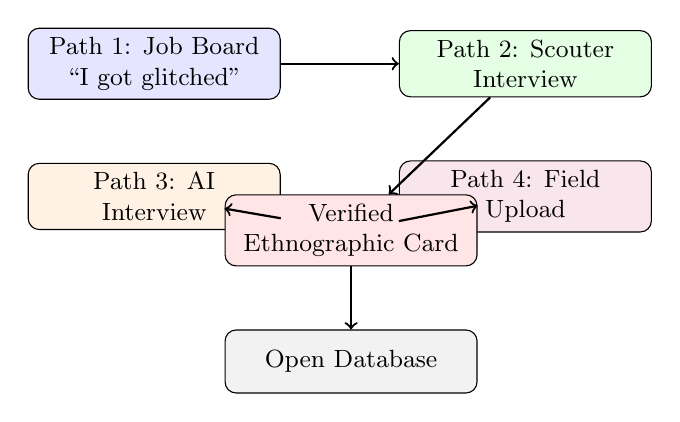
\begin{tikzpicture}[
    node distance=1.2cm,
    box/.style={draw, rounded corners, minimum width=3.2cm, minimum height=0.8cm, align=center, font=\small},
    arrow/.style={->, thick}
]
    \node[box, fill=blue!10] (p1) {Path 1: Job Board\\``I got glitched''};
    \node[box, fill=green!10, right=1.5cm of p1] (p2) {Path 2: Scouter\\Interview};
    \node[box, fill=orange!10, below=0.8cm of p1] (p3) {Path 3: AI\\Interview};
    \node[box, fill=purple!10, right=1.5cm of p3] (p4) {Path 4: Field\\Upload};
    \node[box, fill=red!10, below=1.2cm of p1, xshift=2.5cm] (card) {Verified\\Ethnographic Card};
    \node[box, fill=gray!10, below=0.8cm of card] (db) {Open Database};

    \draw[arrow] (p1) -- (p2);
    \draw[arrow] (p2) -- (card);
    \draw[arrow] (p3) -- (card);
    \draw[arrow] (p4) -- (card);
    \draw[arrow] (card) -- (db);
\end{tikzpicture}
\caption{Four data pathways converging on verified ethnographic cards.}
\label{fig:pathways}
\end{figure}

\textbf{Path 1: Job Board.} The lowest-friction entry point. Anyone can submit a rough report---a brief description of their glitch experience. These reports appear on a public job board visible to Glitch Scouters.

\textbf{Path 2: Scouter Interview (Gold Standard).} A certified Glitch Scouter browses the job board, claims a report, contacts the reporter, and conducts a full semi-structured interview online (via embedded video call or text chat). The session is recorded for verification. This is the highest-quality pathway.

\textbf{Path 3: AI-Conducted Interview.} For immediate self-service, an AI agent conducts the semi-structured interview in real-time on the website. The participant can use text or voice (with automatic speech-to-text transcription). The AI follows the same five-section protocol. A Scouter reviews the output afterward.

\textbf{Path 4: Scouter Direct Upload.} For interviews conducted outside the platform (e.g., at conferences), Scouters upload transcripts and notes directly. A second Scouter peer-reviews.

All four pathways converge on the same output: a \textbf{verified ethnographic card} that enters the open database.

\subsection{The Deliberation Pipeline}

After every interview, regardless of pathway, the raw transcript is processed through a \textbf{deliberation prompt}---an LLM-based transformation that extracts a structured ethnographic card from the unstructured conversation. The prompt enforces strict rules:

\begin{itemize}[noitemsep]
    \item \textbf{Extract, don't invent}: every field must be grounded in what was actually said
    \item \textbf{De-identify everything}: names, employers, locations replaced with generalized descriptions
    \item \textbf{Preserve voice}: participant's own words retained in quotes and emotion descriptions
    \item \textbf{Apply ethological analysis}: Tinbergen's four questions applied as researcher interpretation
    \item \textbf{Transparency}: fields not discussed are explicitly marked as such
\end{itemize}

The generated card then goes through a two-stage human confirmation:

\begin{enumerate}
    \item \textbf{Participant review}: the reporter reviews the rendered card, confirms accuracy, requests changes, or rejects
    \item \textbf{Scouter review}: a certified Scouter verifies de-identification, classification accuracy, and faithfulness to the transcript
\end{enumerate}

No data enters the database without human confirmation.

\section{Glitch Scouters}

Glitch Scouters are certified student interviewers---the human quality layer between raw trust experiences and the database. The certification system itself is a trust mechanism: it ensures data quality through training, calibration, and accountability.

\subsection{Certification Pipeline}

\begin{enumerate}[noitemsep]
    \item \textbf{Application}: statement of interest, relevant background
    \item \textbf{Training}: self-paced module covering protocol, ethogram, and ethics
    \item \textbf{Practice interview}: supervised by PI or senior Scouter
    \item \textbf{Calibration coding}: code 3 sample transcripts, achieve $\kappa \geq 0.6$ against gold standard
    \item \textbf{Certification}: assigned Scouter ID, granted database access
\end{enumerate}

\subsection{Quality Assurance}

Each glitch event is coded by at least two coders. We track Cohen's kappa ($\kappa$) for key categorical fields, targeting $\kappa \geq 0.7$ for glitch type, trust trajectory, and primary affect. Scouters participate in monthly calibration sessions and must maintain reliability standards to retain certification.

\subsection{Scouter Levels}

\begin{table}[h]
\centering
\begin{tabular}{@{}lll@{}}
\toprule
\textbf{Level} & \textbf{Title} & \textbf{Requirements} \\
\midrule
1 & Scout & Certified, $<$10 interviews \\
2 & Pathfinder & 10+ interviews, consistent $\kappa$ \\
3 & Ranger & 25+ interviews, can train new Scouters \\
\bottomrule
\end{tabular}
\caption{Glitch Scouter certification levels.}
\label{tab:scouters}
\end{table}

\section{Technical Architecture}

Trust.Fail is built on a GitHub-native architecture where the repository \textit{is} the database (Figure~\ref{fig:arch}):

\begin{itemize}[noitemsep]
    \item \textbf{GitHub Issues}: glitch reports, interview requests, Scouter applications
    \item \textbf{Pull Requests}: ethnographic cards awaiting confirmation
    \item \textbf{Data directory} (\texttt{data/coded/*.yml}): the canonical database of verified YAML entries
    \item \textbf{GitHub Actions}: automated ethogram generation from structured issue forms
\end{itemize}

The website (\url{https://trust.fail}) is a Next.js application that reads from the GitHub repository, providing browsable, filterable, searchable access to the database. The AI interview system uses the Vercel AI SDK with a large language model API, and embedded video conferencing (Whereby or Daily.co) enables human interviews without leaving the site.

All interviews happen online. Evidence (screenshots, chat logs, recordings) is uploaded and stored alongside the ethnographic card. Consent is obtained digitally via embedded e-signature (DocuSeal), and scheduling uses an embedded booking system (Cal.com).

\section{Ethical Considerations}

Trust.Fail collects sensitive personal accounts and publishes them openly. We identify twelve areas of ethical concern and implement corresponding mitigations:

\begin{enumerate}[noitemsep]
    \item \textbf{Informed consent}: detailed legal waiver, plain-language summaries, opt-in for each data activity, review before publication
    \item \textbf{Re-identification risk}: systematic de-identification, participant review, k-anonymity assessment for unique cases
    \item \textbf{Vulnerable participants}: skip/stop options, interviewer distress training, escalation protocol
    \item \textbf{Power dynamics}: participant reviews card before publication, open questions minimize interviewer influence
    \item \textbf{AI interviewer recursion}: participants can choose human instead; the recursive dynamic is acknowledged as a feature of the research
    \item \textbf{Data misuse}: CC BY 4.0 ensures attribution; responsible use statement accompanies the dataset
    \item \textbf{Cultural bias}: grounded taxonomy, participant-generated categories, multilingual support
    \item \textbf{Scouter welfare}: interview limits, vicarious trauma training, monthly check-ins
    \item \textbf{Incentive effects}: no financial compensation for ``interesting'' stories; dual coding catches fabrication
    \item \textbf{Scope creep}: database is descriptive, not evaluative; positive and negative glitches collected equally
    \item \textbf{Legal compliance}: UK GDPR, Data Protection Act 2018, 30-day withdrawal guarantee, 3-year recording retention
    \item \textbf{Governance}: quarterly ethics review, advisory board to be established before 100 entries
\end{enumerate}

The project will seek ethics approval from the University of Oxford CUREC (Central University Research Ethics Committee).

\section{Related Work}

\subsection{Trust in AI}

The study of trust in AI has a rich history. \citet{lee2004trust} proposed a framework for trust in automation distinguishing performance, process, and purpose. \citet{hoff2015trust} conducted a meta-analysis of factors affecting trust in automation, identifying dispositional, situational, and learned trust. \citet{hancock2011meta} examined how robot, human, and environmental factors influence trust in human-robot interaction. More recently, \citet{jacovi2021formalizing} formalized trust in AI as a relationship between a trustor and trustee with respect to a specific vulnerability.

Trust.Fail differs from this prior work in its emphasis on \textit{naturalistic, incident-based} data rather than controlled experimental measurement. We document trust as a dynamic, situated phenomenon rather than a static attitude.

\subsection{AI Incident Databases}

The AI Incident Database \citep{mcgregor2021preventing} catalogs reported AI failures from media sources. The OECD AI Incidents Monitor tracks policy-relevant AI incidents. Trust.Fail complements these by focusing specifically on \textit{trust dynamics} (not just failures) and collecting data through primary ethnographic interviews rather than secondary media reports.

\subsection{Ethology and Machine Behavior}

\citet{rahwan2019machine} introduced the concept of ``machine behavior,'' arguing that AI systems should be studied using the same behavioral science methods applied to animals and humans. Trust.Fail operationalizes this insight by applying ethological methods---specifically Tinbergen's four questions \citep{tinbergen1963aims}---to the study of trust-relevant AI behaviors.

\subsection{Broad Listening}

\citet{small2023polis} describe ``broad listening'' as technology-assisted processes that help groups understand the distribution of opinions across a population. Trust.Fail applies this principle to trust experiences: by structuring individual glitch reports into a queryable database, we enable researchers to ``listen'' across hundreds of trust experiences simultaneously.

\section{Discussion}

\subsection{Trust.Fail as Research Infrastructure}

Trust.Fail is not a single study but \textbf{research infrastructure}---a platform that enables many studies. The database compounds over time: each new ethnographic card makes the whole corpus more valuable. At sufficient scale ($n > 1000$), the dataset becomes publishable as a flagship resource paper and referenceable as a standard corpus, much as ImageNet became the benchmark for computer vision or the Human Genome Project became the reference for genomics.

\subsection{For AI Safety}

AI safety research urgently needs empirical grounding. Mathematical safety guarantees must account for real failure modes; alignment research must understand how misalignment is actually experienced by users. Trust.Fail provides this empirical foundation---not hypothetical scenarios, but verified accounts of how trust actually breaks, bends, and recovers.

\subsection{For Design and Industry}

Companies building AI products can use Trust.Fail as a reference library: categorized failure patterns, trust benchmarking across AI systems, and design insights traceable to specific architectural and configuration decisions. The ethological analysis is particularly valuable---it reveals not just \textit{what} went wrong but \textit{why}, at the level of mechanism and design lineage.

\subsection{Limitations}

\begin{itemize}[noitemsep]
    \item \textbf{Selection bias}: people who report trust glitches are not a random sample of AI users. The database will overrepresent engaged, reflective users and dramatic incidents.
    \item \textbf{Recall bias}: even with interviews, participants reconstruct events from memory. Evidence uploads (screenshots, logs) partially mitigate this.
    \item \textbf{Cultural coverage}: initial data collection will likely skew toward English-speaking, tech-literate populations. Deliberate outreach to diverse communities is needed.
    \item \textbf{Taxonomy stability}: the seed taxonomy will evolve significantly as data arrives. Early analyses should treat categories as provisional.
    \item \textbf{AI interviewer quality}: AI-conducted interviews may miss nuances that human Scouters would catch. Comparative analysis of interview quality across pathways is planned.
\end{itemize}

\section{Roadmap}

\begin{itemize}[noitemsep]
    \item \textbf{Year 1}: Build protocol and website, train initial Scouters, collect first 100--200 ethnographic cards. Publish methodology paper (target: CHI, CSCW, or FAccT).
    \item \textbf{Year 2--3}: Scale to 1,000+ cards. Emergent taxonomy stabilizes. Cross-cultural patterns appear. Dataset paper targeting Nature Human Behaviour or Science.
    \item \textbf{Year 3+}: Trust.Fail becomes a standard reference dataset for trust in human-AI interaction. Continuously growing. Cited across AI safety, HCI, STS, and policy.
\end{itemize}

\section{Conclusion}

Trust is the critical yet underexamined substrate of human-AI interaction. Trust.Fail provides a systematic, open method for documenting trust glitches as they occur in the wild, combining ethnographic richness with ethological rigor. By building an openly licensed, continuously growing database of verified trust experiences, we aim to provide the empirical foundation that AI safety, HCI, and trust research currently lacks.

The project is open-source and available at \url{https://github.com/realitydeslab/tx-glitch}. The database is accessible at \url{https://trust.fail}. We invite researchers, students, and anyone who has experienced a trust glitch to contribute.

\section*{Acknowledgments}

This work is supported by Reality Design Lab at the University of Oxford. We thank the open-source community and early contributors to the Trust.Fail project.

\bibliographystyle{plainnat}
\bibliography{references}

\end{document}
